\subsection{Training data} \label{supervised_approach_data}

In this section, we present the subset of \acrshort{mag} documents, which we use to train the supervised models. We first present how we have retrieved documents from the OpenAlex \acrshort{api} in section \ref{supervised_approach_data_retrieval}. We retrieve up to 100 documents for each subject in our subset, ensuring that each document has an abstract.

Then, in section \ref{supervised_approach_data_hierarchy}, we analyze the subject assignments of the documents. We focus on the consistency of the assignments regarding the hierarchy. If a document is assigned a subject, it should also have all its ancestors assigned. This is relevant for the model training, as hierarchy violations hinder the model's understanding of the subjects \cite{gargiulo2019deep}.

Finally, in section \ref{supervised_approach_data_result}, we discuss the resulting dataset. We have gathered over 200,000 documents. After correcting hierarchy violations, it comprises almost 2 million subject assignments. Only two subjects are not assigned to any documents, out of the 2,157 included in our subset.

\subsubsection{Document retrieval} \label{supervised_approach_data_retrieval}

To retrieve documents from OpenAlex, we iterate over the subjects in our subset of \acrshort{mag} subjects and look for journal articles that include each subject. We iterate over the resulting documents, and keep those that have an abstract and were not previously retrieved through another subject. The abstract of the documents is given as an inverted index, where each word is mapped to its positions in the abstract. This was done for copyright reasons.

We have retrieved up to 100 documents per subject, and stored them in multiple files, with max. 3,000 documents per file. For each document, we first build the abstract and append it to the title. We then process the resulting text, and store it in a file together with its assigned subjects. The processing involves tokenizing and lemmatizing the data, just as it was done for the texts of the repositories (see section \ref{implementation_vocab}). We also discard stopwords and tokens that have less than three letters, which removes numbers, symbols and quantities (e.g. 100mg).

\subsubsection{Hierarchy violations} \label{supervised_approach_data_hierarchy}

Here we look at the subject assignments of the documents presented above, looking for inconsistencies regarding the hierarchy of subjects, before presenting the final training dataset. The assignments of a document are inconsistent if the ancestors of an assigned subject are not assigned as well. We consider this a violation of the hierarchy.

There are 1,952 documents that are not assigned a \acrshort{mag} field, which are therefore inconsistent, as they are assigned subjects of further levels but not from the first. Interestingly, 122 of these documents have the subject \textit{Mechanics} assigned to them. 427 of these documents without assigned fields only have one assigned subject. On average, these subjects are assigned 1.2 subjects, with 1,582 distinct subject assignments. We have corrected these violations using the lists of ancestors of the subjects. The resulting dataset is presented in the next section.

\subsubsection{Resulting dataset} \label{supervised_approach_data_result}

\begin{figure}
    \centering
    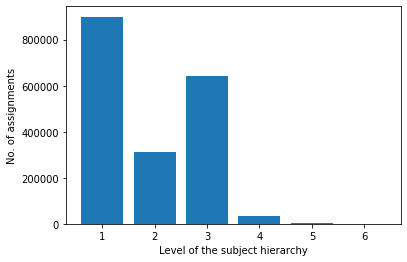
\includegraphics[width=.7\textwidth]{figures/supervised_approach/training_data_levels.png}
    \caption{Number of subject assignments per hierarchy level.}
    \label{fig:training_data_levels}
\end{figure}

Following the retrieval procedure outlined above, we could gather 214,538 documents, comprising 100 documents for all subjects except for 17. When looking at all assignments, there are two subjects of our subset for which we could not retrieve any documents: \textit{Algorithm design} and \textit{Premise}. There are two further subjects for which we could not retrieve any documents (\textit{Shoot} and \textit{Intensive care unit}), but they are present in more than 300 documents each, when looking at the whole dataset. This occurs because the only documents that include these subjects were already retrieved by looking at the documents assigned with other subjects.

In total, there are 1,890,080 subject assignments. 821,273 of these assignments were added to fix hierarchy violations. The field that has benefited the most from fixing the hierarchy violations is \textit{Engineering}, which went from being the field with the least assignments (2,565), to having over 60,000 assignments. All fields have more than 20,000 assignments after the corrections, whereas before there were several with less than 5,000 assignments.

As shown in \ref{fig:training_data_levels}, most of them belong to the first hierarchy level. Here, only the field assignments are considered. \textit{Biology} is the most assigned field, with over 80,000 assignments. \textit{Art} has the least assignments, with just over 20,000. Among the other levels of the hierarchy, the most popular subjects are \textit{Law}, with 49,842 assignments and \textit{Ecology}, with 37,136 assignments. Both had less than 10,000 assignments before fixing the hierarchy violations.

Although we have avoided duplicates by keeping the OpenAlex IDs of the retrieved documents, there are 4,849 documents with the same data. 122 of them are documents for which no tokens remained after the filtering procedure, and 31 of them have uninformative texts like review appeals. The remaining documents are actual duplicates, with the same data appearing in at most three documents. There are 2,346 distinct documents among them, with an average of one duplicate per document. Thus, the final number of distinct documents is 212,035.

\begin{figure}
    \centering
    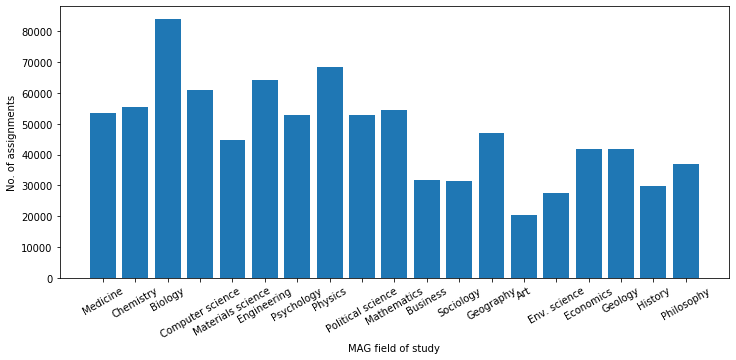
\includegraphics[width=\textwidth]{figures/supervised_approach/training_data_fields.png}
    \caption{Distribution of the documents across the MAG fields of study.}
    \label{fig:training_data_fields}
\end{figure}